\chapter{Introduction}
\label{chap:intro}

\section{Motivation}
\label{sect:motivation}
LiDAR sensors provide critical depth information for autonomous driving and robotics. LiDAR intensity maps are often sparse and incomplete. Using depth maps as additional input is a way to improve the richness and accuracy of LiDAR prediction. The Pix2Pix image-to-image translation network is a promising approach for integrating these modalities \cite{CycleGAN2017} \cite{isola2017image}.
\section{Contribution}
This project explores the use of the Pix2Pix network to predict LiDAR intensity maps using RGB images and depth maps as additional inputs.
\section{Related work}
\textbf{BP-Net (Bilateral Propagation Network):} BP-Net is a neural network architecture designed for depth completion tasks. It generates dense depth maps from sparse data \cite{BP-Net}. \\
\newline \textbf{Depth-Anything Models:}  Depth-Anything represents a significant advance in monocular depth estimation by using both labelled and unlabelled data on a large scale \cite{depthanything}. There are two versions available, the second having better accuracy and robustness of depth estimation \cite{depth_anything_v2}. These nets are also capable of performing metric depth to provide distance measurements from images.
\\ \textbf{3D Reconstruction Techniques:} 3D reconstruction focuses on creating three-dimensional models from two-dimensional images or depth data. 3D reconstruction techniques include methods such as structure-from-motion (SfM) and multi-view stereo (MVS). These techniques aim to generate accurate 3D representations of scenes or objects from multiple views or depth sensors \cite{saxena2008depth}.

%\chapter{Preparations}
%used google colab, pix2pix network getting the right input, pix2pix problems



\chapter{LiDAR Intensity Prediction} %from RGB and Depth Images}
\section{Setup}
First, the depth was created using RGB images from "The KITTI Dataset" \cite{Geiger2013IJRR}. In order to get a large variety of depths for comparison, the Bilateral Propagation Network (BP-Net), Depth-Anything v1 \& 2 and Metric v2 were used. The metric depth v1 was not used because it did not run in time.
\subsection{Bilateral Propagation Net (BP-Net)}
\begin{itemize}
	\item \textbf{Purpose:} Used for depth completion to improve depth maps from incomplete or noisy data.
	\item \textbf{Data set:} The input was raw data from kitti with a depth completion set already available. 
\end{itemize}

\subsection{Depth-Anything Models}
\begin{itemize}
	\item \textbf{Depth-Anything v1:} Provides initial depth estimates using large unlabeled data for zero-shot learning.
	\item \textbf{Depth-Anything v2:} Enhanced depth prediction capabilities, incorporating improvements over v1 for better depth map accuracy.


 	\item \textbf {Metric Depth Estimation v2:} Enhanced depth maps with precise metric depth measurements.

	\item \textbf{Dataset:} Corresponding RGB images that were used in BP-Net for better comparison.
\end{itemize}

\subsection{Pix2pix Network}
\begin{itemize}
	\item \textbf{Purpose:} Image-to-Image processing to predict LiDAR intensity from RGB and depth images. 
	\item \textbf{Training Data:} RGB from the KITTI dataset and their created depth pairs.
	Eight different input data variations were used, see in section \ref{results}.
\end{itemize}

\section{Implementation}
\subsection{Generation of depth maps}
\begin{itemize}
	\item \textbf{BP-Net:} An existing pre-trained model on Kitti data was loaded. The BP-Net model was applied to generate depth maps from the KITTI dataset. The output was 1000 depth maps.
	
	\item \textbf{Depthanthing v1 \& 2 and metric depth:} The depth networks also provide trained models for kitti. There are three versions of all depth nets. The small, the base and the large model. For similar results the base model was loaded in every case.   
	
	\item \textbf{Dataset preparation:} RGB images were paired with the generated depth maps to create a comprehensive training dataset for the pix2pix model.
	\end{itemize}
\begin{figure}[!ht]
	\centering
	%\scalebox{2}[1]{\includegraphics[width=0.2\textwidth]{abb/rgb/0000000030.png}}
	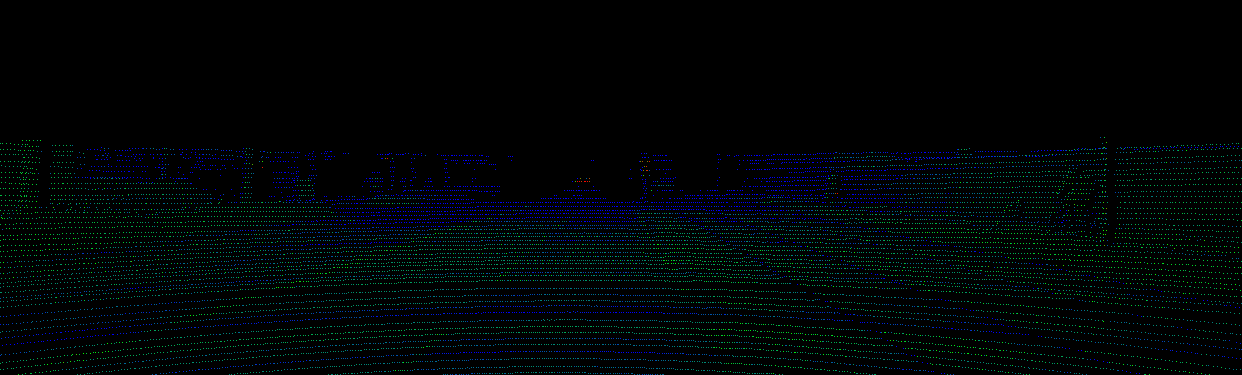
\includegraphics[width=0.5\textwidth]{abb/network/0000000077.png}
	\includegraphics[width=0.5\textwidth]{abb/network/0000000077bp.png}
	\includegraphics[width=0.5\textwidth]{abb/network/0000000077v1.png}
	\includegraphics[width=0.5\textwidth]{abb/network/0000000077v2.png}
	\includegraphics[width=0.5\textwidth]{abb/network/0000000077metric.png}
	\caption{RGB and created depth (BP, Deptanything v1,2 and metric v2)}
	\label{all_depths}
\end{figure}
The four depth maps sources (shown in figure \ref{all_depths}) have different properties. The BP-Net has very little near-field resolution. The Depth-Anything depth maps are both more dense in the near field, but lack the distant objects. Version 2 has better edge visualisations and some distant objects like the sign on the left or the car are better visible. The metric depth has the best focus on the far field, but has very little  information in near field. 

\newpage
\subsection{Model Training}\label{modeltraining}
\begin{itemize}
	\item \textbf{Pix2pix configuration:} The pix2pix architecture was modified to accept RGB images and depth maps (4 dim.) as inputs to be able to scan the input channel seperately and to avoid losses due to overlaying RBG and depth images. The unmodified pix2pix was trained to predict LiDAR intensity values based on depth maps inputs. The 4 dimensional pix2pix was given the input of rgb plus depth maps.
	\item \textbf{Training process:} Training parameters such as learning rate 0.0002000, batch size 1, and number of epochs 20 were set. The model was trained using the prepared dataset in the configuration 1000 images divided into 800 training, 100 validation, 100 test folders. The input is different for the sole depth input and the RGBD input because the script for dividing are not executed in the same way. This was discovered after the training and test runs. Both versions were run with masked out the pixel value -1 to reduce the areas of no interest. The input was cropped to a size of $256 \times 256$  but not scaled.
\end{itemize}

\section{Results} \label{results}
% wandb didnt work so no loss curves availble

%\newline
This section presents the results of the experiments using different setups to predict LiDAR intensity. The performance of several methods was evaluated, including the separate depths from BP-Net, Depth-Anything v1 and v2, and metric depth estimation to LiDAR. The other four are RGB plus each of these depths to LiDAR. The images returned are crop and the full versions are shown for comparison. The cropped version is the right part of the full resolution ($1216 \times 352$) images. For the 4 dimensional runs, the cropped LiDAR groundtruth is used for better visualisation as this pix2pix version gives these additional outputs. The results of eight runs are summarised below.
%\newpage
\subsection{Depth BP-Net to LiDAR}

Using only the depth maps generated by BP-Net (Figure \ref{bp_results}), without accompanying RGB images, the model was trained to predict LiDAR intensity. This approach resulted in some visible predictions.
\begin{figure}[!ht]
	\centering
	%\scalebox{2}[1]{\includegraphics[width=0.2\textwidth]{abb/rgb/0000000030.png}}
	\includegraphics[width=0.4\textwidth]{abb/singleruns/bp/depth/0000000070.png}
	\includegraphics[width=0.4\textwidth]{abb/singleruns/bp/lidar/0000000070.png}
	\includegraphics[width=0.3\textwidth]{abb/singleruns/bp/result/0000000070.png}
	\caption{Depth BP-Net LiDAR and predicted LiDAR.}
	\label{bp_results}
\end{figure}
\newpage
\subsection{Depth-Anything v1 to LiDAR}

The Depth-Anything v1 model (Figure \ref{v1_results}) provided initial depth estimates using large-scale unlabelled data. When used to predict LiDAR intensity, this model showed results that are more in line with depth maps rather than LiDAR intensity.
\begin{figure}[!ht]
	\centering
	%\scalebox{2}[1]{\includegraphics[width=0.2\textwidth]{abb/rgb/0000000030.png}}
	\includegraphics[width=0.4\textwidth]{abb/singleruns/v1/depth/0000000070.png}
	\includegraphics[width=0.4\textwidth]{abb/singleruns/v1/lidar/0000000070.png}
	\includegraphics[width=0.3\textwidth]{abb/singleruns/v1/result/0000000070_depth.png}
	\caption{Depth Depth-Anything v1 LiDAR and predicted LiDAR.}
	\label{v1_results}
\end{figure}
\newpage
\subsection{Depth-Anything v2 to LiDAR}

The Depth-Anything v2 (Figure \ref{v2_results}) shows almost the same result as v1. It could be that pix2pix was trying to learn LiDAR to depth, but the datasets and the training settings were correct for that.
\begin{figure}[!ht]
	\centering
	%\scalebox{2}[1]{\includegraphics[width=0.2\textwidth]{abb/rgb/0000000030.png}}
	\includegraphics[width=0.4\textwidth]{abb/singleruns/v2/depth/0000000070.png}
	\includegraphics[width=0.4\textwidth]{abb/singleruns/v2/lidar/0000000070.png}
	\includegraphics[width=0.3\textwidth]{abb/singleruns/v2/result/0000000070.png}
	\caption{Depth-Anything v2 LiDAR and predicted LiDAR.}
	\label{v2_results}
\end{figure}
\newpage
\subsection{Metric Depth to LiDAR}
In this approach, accurate metric depth measurements (Figure \ref{metric_results}) were used to predict LiDAR intensity. This method significantly shows a good prediction of LiDAR intensity.
\begin{figure}[!ht]
	\centering
	%\scalebox{2}[1]{\includegraphics[width=0.2\textwidth]{abb/rgb/0000000030.png}}
	\includegraphics[width=0.4\textwidth]{abb/singleruns/metricv2/depth/0000000070.png}
	\includegraphics[width=0.4\textwidth]{abb/singleruns/metricv2/lidar/0000000070.png}
	\includegraphics[width=0.3\textwidth]{abb/singleruns/metricv2/result/0000000070.png}
	\caption{Metric depth LiDAR and predicted LiDAR.}
	\label{metric_results}
\end{figure}
\newpage	
\subsection{RGB plus BP-Net to LiDAR}
In this setup (Figure \ref{bp_rgbd}), RGB images were combined with depth maps generated by the BP-Net model to predict LiDAR intensity. The integration of depth information from BP-Net shows a significant increase in prediction accuracy compared to using depth map images alone. For example, the cars are barely visible and the background is almost incorrectly filled, perhaps due to masking.
\begin{figure}[!ht]
	\centering
	% Erstes Bild
	\begin{subfigure}{0.4\textwidth}
		\centering
		\includegraphics[width=\linewidth]{abb/plusdepthruns/bp/rgb/0000000069.png}
		\caption{RGB Image}
		\label{bp_rgbd1}
	\end{subfigure}
	
	\vspace{1em} % Vertikaler Abstand zwischen den Bildern
	
	% Zweites Bild
	\begin{subfigure}{0.4\textwidth}
		\centering
		\includegraphics[width=\linewidth]{abb/plusdepthruns/bp/depth/0000000069.png}
		\caption{Depth Map}
		\label{bp_rgbd2}
	\end{subfigure}
	
	\vspace{1em} % Vertikaler Abstand zwischen den oberen und unteren Bildern
	
	% Drittes und viertes Bild nebeneinander
	\begin{subfigure}{0.25\textwidth}
		\centering
		\includegraphics[width=\linewidth]{abb/plusdepthruns/bp/result/0000000069_real_B.png}
		\caption{Groundtruth LiDAR}
		\label{fig:bp_pred_lidar}
	\end{subfigure}
	%hfill
	\begin{subfigure}{0.25\textwidth}
		\centering
		\includegraphics[width=\linewidth]{abb/plusdepthruns/bp/result/0000000069_fake_B.png}
		\caption{Predicted LiDAR}
		\label{fig:bp_fake_lidar}
	\end{subfigure}
	
	\caption{RGB, Depth, Predicted LiDAR, and Predicted LiDAR images for the BP-Net setup.}
	\label{bp_rgbd}
\end{figure}
\newpage
\subsection{RGB plus Depth-Anything v1 to LiDAR}
When RGB images were combined with depth maps from Depth-Anything v1 (Figure \ref{v1_rgbd}), the model performed better than using depth alone. The fusion of RGB and depth data provided a more comprehensive input, resulting in a LiDAR intensity that is close to the ground truth. The end of the road is visible.
\begin{figure}[!ht]
	\centering
	% Erstes Bild
	\begin{subfigure}{0.4\textwidth}
		\centering
		\includegraphics[width=\linewidth]{abb/plusdepthruns/v1/rgb/0000000070.png}
		\caption{RGB Image}
		\label{fig:v1_rgb}
	\end{subfigure}
	
	\vspace{1em} % Vertikaler Abstand zwischen den Bildern
	
	% Zweites Bild
	\begin{subfigure}{0.4\textwidth}
		\centering
		\includegraphics[width=\linewidth]{abb/plusdepthruns/v1/depth/0000000070.png}
		\caption{Depth Map}
		\label{fig:v1_depth}
	\end{subfigure}
	
	\vspace{1em} % Vertikaler Abstand zwischen den oberen und unteren Bildern
	
	% Drittes und viertes Bild nebeneinander
	\begin{subfigure}{0.25\textwidth}
		\centering
		\includegraphics[width=\linewidth]{abb/plusdepthruns/v1/result/0000000070_real_B.png}
		\caption{Groundtruth LiDAR}
		\label{fig:v1_pred_lidar}
	\end{subfigure}
	%hfill
	\begin{subfigure}{0.25\textwidth}
		\centering
		\includegraphics[width=\linewidth]{abb/plusdepthruns/v1/result/0000000070_fake_B.png}
		\caption{Predicted LiDAR}
		\label{fig:v1_fake_lidar}
	\end{subfigure}
	
	\caption{RGB, Depth, LiDAR, and Predicted LiDAR images for the Depth-Anything v1 setup.}
	\label{v1_rgbd}
\end{figure}
\newpage
\subsection{RGB plus Depth-Anything v2 to LiDAR}
RGB images paired with Depth-Anything v2 depth maps (Figure \ref{v2_results}) show better prediction than v1. The sign in the ground  truth is more visible due to the better depth map resolution of Depth-Anything v2.
\begin{figure}[!ht]
	\centering
	% Erstes Bild
	\begin{subfigure}{0.4\textwidth}
		\centering
		\includegraphics[width=\linewidth]{abb/plusdepthruns/v2/rgb/0000000070.png}
		\caption{RGB Image}
		\label{fig:v2_rgb}
	\end{subfigure}
	
	\vspace{1em} % Vertikaler Abstand zwischen den Bildern
	
	% Zweites Bild
	\begin{subfigure}{0.4\textwidth}
		\centering
		\includegraphics[width=\linewidth]{abb/plusdepthruns/v2/depth/0000000070.png}
		\caption{Depth Map}
		\label{fig:v2_depth}
	\end{subfigure}
	
	\vspace{1em} % Vertikaler Abstand zwischen den oberen und unteren Bildern
	
	% Drittes und viertes Bild nebeneinander
	\begin{subfigure}{0.25\textwidth}
		\centering
		\includegraphics[width=\linewidth]{abb/plusdepthruns/v2/result/0000000070_real_B.png}
		\caption{Groundtruth LiDAR}
		\label{fig:v2_pred_lidar}
	\end{subfigure}
	%hfill
	\begin{subfigure}{0.25\textwidth}
		\centering
		\includegraphics[width=\linewidth]{abb/plusdepthruns/v2/result/0000000070_fake_B.png}
		\caption{Predicted LiDAR}
		\label{v2}
	\end{subfigure}
	
	\caption{RGB, Depth, LiDAR, and Predicted LiDAR images for the Depth-Anything v2 setup.}
	\label{v2_rgbd}
\end{figure}
\subsection{RGB plus Metric Depth to LiDAR}

The combination of accurate metric (Figure \ref{metric_rgbd}) depth measurements produced the most accurate predictions of LiDAR intensity. This setup exploited the strengths of both RGB data and metric depth and gave the best results in all runs. The contours of the cars are visible on the right. 

\begin{figure}[!ht]
	\centering
	
	% Erstes Bild
	\begin{subfigure}{0.4\textwidth}
		\centering
		\includegraphics[width=\linewidth]{abb/plusdepthruns/metricv2/rgb/0000000417.png}
		\caption{RGB}
		\label{fig:bild1}
	\end{subfigure}
	
	\vspace{1em} % Vertikaler Abstand zwischen den Bildern
	
	% Zweites Bild
	\begin{subfigure}{0.4\textwidth}
		\centering
		\includegraphics[width=\linewidth]{abb/plusdepthruns/metricv2/depth/0000000417.png}
		\caption{Depth}
		\label{fig:bild2}
	\end{subfigure}
	
	\vspace{1em} % Vertikaler Abstand zwischen den oberen und unteren Bildern
	
	% Drittes und viertes Bild nebeneinander
	\begin{subfigure}{0.25\textwidth}
		\centering
		\includegraphics[width=\linewidth]{abb/plusdepthruns/metricv2/result/0000000417_real_B.png}
		\caption{Groundtruth LiDAR}
		\label{fig:bild3}
	\end{subfigure}
	%%hfill
	\begin{subfigure}{0.25\textwidth}
		\centering
		\includegraphics[width=\linewidth]{abb/plusdepthruns/metricv2/result/0000000417_fake_B.png}
		\caption{Predicted LiDAR}
		\label{fig:bild4}
	\end{subfigure}
	
	\caption{RGB, Depth-Anything metric, LiDAR and predicted LiDAR.}
	\label{metric_rgbd}
\end{figure}
\chapter{Conclusion}
In conclusion, the results of the different depth maps against LiDAR show poor prediction for most of the single depthmap inputs. The combined inputs perform better in prediction. The comparisons are not fully acceptable because there were problems with the different output images and mostly not matching samples. Also, the supplied script did not work for this evaluation because the cropped output image should be stitched together in pairs of 4 to get the full image. This makes it difficult to analyse the data. \newline \\Overall, there are some differences to note: Depth-Anything v2 performs better than v1, and metric depth is better than both. The BP network also shows some good results. A better approach is to use the same output images and run without masking for a more reliable result. Also, the lack of loss function due to non-working scripts and not tracked by wandb is a big disadvantage for evaluation. 
\newpage
\chapter{Appendix}
\subsection{RGB to LiDAR}

These are the results for the pix2pix model trained using only RGB images to predict LiDAR intensity. The predicted LiDAR appears to be good, but to focus more on the different depths, this has been omitted.
\begin{figure}[!ht]
	\centering
	%\scalebox{2}[1]{\includegraphics[width=0.2\textwidth]{abb/rgb/0000000030.png}}
	\includegraphics[width=0.4\textwidth]{abb/singleruns/rgb/rgb/0000000070.png}
	\includegraphics[width=0.4\textwidth]{abb/singleruns/rgb/LiDAR/0000000030.png}
	\includegraphics[width=0.3\textwidth]{abb/singleruns/rgb/result/0000000070.png}
	\caption{RGB LiDAR and predicted LiDAR.}
	\label{rgb}
\end{figure}


%\section{References}
%bp net work pix2pix depth anything v1 2 paper for them  some for LiDAR intensity
